\documentclass[12pt,a4paper]{article}
\usepackage[UTF8]{ctex}
\usepackage{amsmath,amssymb}
\usepackage{listings}
\usepackage{xcolor}
\usepackage{hyperref}
\usepackage{geometry}
\usepackage{graphicx}
\geometry{margin=2.5cm}

\lstdefinestyle{python}{
  language=Python,
  basicstyle=\ttfamily\small,
  keywordstyle=\color{blue}\bfseries,
  commentstyle=\color{gray},
  stringstyle=\color{red},
  showstringspaces=false,
  breaklines=true,
  frame=single,
  backgroundcolor=\color{gray!10}
}

\title{E91 Quantum Key Distribution / E91 量子密钥分发}
\author{QuoNic}
\date{}

\begin{document}
\maketitle

\begin{center}
\textbf{Communication / 通信} | 难度：高级 | 预计时间：20 分钟
\end{center}

\tableofcontents
\newpage

\section{为什么需要？}

E91 是基于纠缠的量子密钥分发协议，比 BB84 更安全。

\subsection{经典局限}
\b\begin{itemize}
  \item BB84 需要可信的量子源
  \item BB84 无法检测中间人攻击
\end{itemize}

\subsection{量子优势}
\b\begin{itemize}
  \item E91 使用纠缠态，不需要可信量子源
  \item 可以通过 Bell 不等式检测窃听
  \item 提供无条件安全性
\end{itemize}

\subsection{实际应用}
\b\begin{itemize}
  \item 量子密钥分发网络
  \item 量子安全通信
  \item 量子互联网
\end{itemize}

\section{快速上手}

\begin{lstlisting}[style=python]
from quonic.algorithms import e91

# Run E91 protocol
result = e91(n_bits=100, noise=0.0)
print(f"Shared key: {result.key}")
print(f"Bell violation: {result.bell_violation}")
\end{lstlisting}

\textbf{预期输出}：
\begin{verbatim}
Shared key: 01101001...
Bell violation: 2.828
\end{verbatim}

\section{原理详解}

\subsection{电路图}

\begin{center}
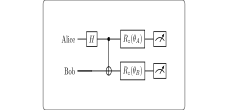
\includegraphics[width=0.6\textwidth]{../../images/e91_circuit.svg}
\end{center}

\subsection{数学推导}

E91 协议使用 Bell 态：
\begin{equation}
|\Phi^+\rangle = \frac{|00\rangle + |11\rangle}{\sqrt{2}}
\end{equation}

\textbf{协议步骤}：
\begin{enumerate}
  \item 源产生 Bell 对，分发给 Alice 和 Bob
  \item Alice 和 Bob 随机选择测量基
  \item 公开比较测量基
  \item 保留基相同的比特作为密钥
  \item 用 Bell 不等式检测窃听
\end{enumerate}

\textbf{Bell 不等式}：
\begin{equation}
S = |E(a,b) - E(a,b') + E(a',b) + E(a',b')| \leq 2
\end{equation}

量子力学预测 $S = 2\sqrt{2} \approx 2.828$。

\subsection{几何解释}

E91 利用纠缠的非局域性，通过 Bell 不等式验证量子关联，从而检测窃听。

\section{代码详解}

\begin{lstlisting}[style=python]
from quonic.algorithms import e91

# e91(n_bits, noise)
# n_bits: number of bits to generate
# noise: channel noise rate
result = e91(n_bits=100, noise=0.0)

# result.key: shared secret key
# result.bell_violation: Bell inequality violation
# result.error_rate: quantum bit error rate
print(f"Key: {result.key}")
print(f"Bell violation: {result.bell_violation}")
\end{lstlisting}

\section{进阶用法}

\subsection{场景 1：带噪声的 E91}

\begin{lstlisting}[style=python]
# E91 with noise
result = e91(n_bits=100, noise=0.05)
print(f"Bell violation: {result.bell_violation}")
# If violation < 2, channel may be compromised
\end{lstlisting}

\subsection{场景 2：窃听检测}

\begin{lstlisting}[style=python]
# Eavesdropping detection
result = e91(n_bits=100, noise=0.0)
if result.bell_violation > 2:
    print("Channel is secure")
else:
    print("Eavesdropper detected!")
\end{lstlisting}

\section{适用场景}

\subsection{量子密钥分发网络}

E91 可以用于构建量子密钥分发网络。

\subsection{量子安全通信}

E91 提供无条件安全性，适用于高安全需求的通信。

\section{常见问题}

\subsection{E91 和 BB84 有什么区别？}

E91 使用纠缠态，BB84 使用单光子。E91 可以通过 Bell 不等式检测窃听。

\subsection{E91 的安全性如何？}

E91 提供无条件安全性，基于量子力学的基本原理。

\section{学习路径}

\subsection{前置知识}
\b\begin{itemize}
  \item Bell 态
  \item Bell 不等式
  \item 量子测量
\end{itemize}

\subsection{继续学习}
\b\begin{itemize}
  \item 量子中继
  \item 量子互联网
  \item 量子密码学
\end{itemize}

\section{完整示例代码}

\subsection{示例 1：基本 E91}

\begin{lstlisting}[style=python]
from quonic.algorithms import e91

result = e91(n_bits=100, noise=0.0)
print(f"Key: {result.key}")
\end{lstlisting}


\section{下载}

\begin{itemize}
  \item [e91.py](https://github.com/ChrisLee0721/QuoNic/blob/main/examples/e91/e91.py)
\end{itemize}

\end{document}
